\section{Проблемы реализации алгоритмов асимметричного шифрования и пути их
решения}

При построении корпоративных систем электронного документооборота, основанных на
асимметричных алгоритмах шифрования, неизбежно возникает ряд проблем, связанных
с реализацией математического решения криптографических функций разрабатываемого
комплекса.

\subsection{Представление чисел в криптографических алгоритмах с открытым
ключом} 

Несмотря на то, что с виду алгоритм достаточно не сложен в реализации,
для вычисления всех параметров необходимо произвести большой объём операций. Это
связано с тем, что параметры всех формул алгоритма -- довольно  длинные числа
(примерно $ 2^{1024} $), и для осуществления простейших операций над ними
необходим специальный модуль работы  с  большими числами, так как стандартные типы данных
не позволяют вместить такие числа.~\cite{ECP}
Числа, для представления которых в стандартных компьютерных типах данных не
хватает количества двоичных разрядов, называются <<длинными>>. Реализация
арифметических операций над такими <<длинными>> числами имеет название <<длинной
арифметики>>.

Организация работы с <<длинными>> числами во многом зависит от их представления.
<<Длинное>> число можно записать, например, с помощью массива десятичных цифр,
количество элементов в таком массиве равно количеству значащих цифр в
<<длинном>> числе. При реализации арифметических операций над этим числом,
размер массива должен быть достаточным, чтобы разместить в нем и результат, например, результат
операции умножения.

Существуют и другие представления <<длинных>> чисел. Рассмотрим одно из них.
Представим наше число
\begin{center}
$30! = 265252859812191058636308480000000$
\end{center} в виде:
\begin{center}
$30! = 2 * (10^4)^8 + 6525 * (10^4)^7 + 2859 * (10^4)^6 + 8121 * (10^4)^5 + 9105
* (10^4)^4 + 8636 * (10^4)^3 + 3084 * (10^4)^2 + 8000 * (10^4)^1 + 0000 *
(10^4)^0$
\end{center}

Это представление наталкивает на мысль о массиве, представленном в таблице
~\ref{tab:2}.

\begin{table}[ht]
  \centering
  \small
  \begin{tabular}{|p{4cm}|*{10}{c|}}
    \hline
	\textbf{Номер элемента в массиве}  & 0 & 1 & 2 & 3 & 4 & 5 & 6 & 7 & 8 & 9 \\
	\hline 
	\textbf{Значение} & 9 & \ \ \ 0 & 8000 & 3084 & 8636 & 9105 & 8121 & 2859 &
	6525 & \ \ \ 2
	\\
	\hline
  \end{tabular}
  \caption{Представление числа}
  \label{tab:2}
\end{table}

Мы можем считать, что наше <<длинное>> число представлено в 10000-10 системе
счисления (десятитысячно-десятичная система счисления, приведя аналогию с
восьмерично-десятичной системой счисления), а <<цифрами>> числа являются
четырехзначные числа. В целях ускорения вычислений выгодно брать за основание
системы счисления, в которой будет храниться «длинное» число, равное максимально
допустимому числу одного из стандартных типов данных ($2^{16} = 65536$).
В нулевом элементе массива хранится длина числа или количество используемых
ячеек в массиве. Для удобства дальнейшей работы цифры числа будут храниться в
обратном порядке. Для совершения простейших операций над такими числами
необходимо применять алгоритмы сложения, вычитания, умножения и деления
<<столбиком>>.

\subsection{Определение <<простоты>> числа}
Задача определения простоты чисел является неотъемлемой частью реализации
асимметричных алгоритмов шифрования.

Неудовлетворительное решение данной задачи может сильно повлиять на защищённость
данных. Напомним, что число называется простым, если не имеет целых делителей
кроме единицы и самого себя.  При традиционном подходе достаточно поделить число
m по порядку на все числа от 2 до m-1, тогда число m можно считать простым в
случае неделимости на цело ни на одно из предложенных. Учитывая, что в
алгоритмах шифрования используются <<длинные>> числа (порядка $2^{1024}$),
подобный подход становиться вычислительно неосуществимой задачей.
В этом случае можно прибегнуть к малой теореме Ферма, которая гласит, что при
условии простоты p и любом b выполняется равенство 
\begin{center}
$b^{p-1} \equiv 1 \ (mod \ p)$.
\end{center}
Обобщение и доказательство приводятся в источнике.~\cite{ferma}

На примере числа 341, являющееся не простым, 341 = 11 * 31, равенство то же
выполняется.

$2^{340} \equiv 1 \ (mod \ 341)$ (действительно, $2^{340} = (2^{10})^{34} =
1024^{34}$, но $1024 = 3 * 341 + 1 \equiv 1 \ (mod \ 341)$, поэтому $1024^{34} \equiv 1
\ (mod \ 341)$).

Более того, существуют числа, которые не являются простыми, но которые ведут
себя как простые в малой теореме Ферма. Такие числа называются кармайкловыми, то
есть числа, являющиеся взаимно простыми с b, при которых выполняется условие
малой теоремы Ферма.

Модификация данной теоремы, предложенная Рабином, применима к любым целым
числам.

Тест Рабина является вероятностным. Для входного целого числа m тест Рабина
может выдать один из следующих двух ответов:
\begin{enumerate}
  \item Число m является составным;
  \item Не знаю.
\end{enumerate}

В случае первого ответа число m действительно является составным, тест Рабина
предъявляет доказательство этого факта. Второй ответ может быть выдан как для
простого, так и для составного числа m. Однако для любого составного числа m
вероятность второго ответа не превышает $\frac{1}{4}$. Ценность теста Рабина
состоит именно в неравенстве, ограничивающем сверху вероятность второго ответа для
произвольного составного числа m.
При проведении N тестов с составным числом m, в результате которых получаем
второй ответ из двух возможных,  вероятность того, что число m - составное не
превышает  $\frac{1}{4}N$ . При $N \rightarrow \infty$  вероятность этого факта
стремиться к нулю.

Тем не менее, тест Рабина не предъявляет доказательства того, что число m простое.
Доказательство законности теста Рабина и алгоритм его работы приведены в
источнике.~\cite{rabin}

\subsection{Генерация случайных чисел}
В криптографических алгоритмах с открытым ключом требуется <<длинное>> случайное
число, генерируемое каждый раз, когда необходимо зашифровать данные.

В качестве генератора случайного или неожиданного числа предлагается взять
механизм, основанный на случайном действии подписчика документа. Такой способ
получения случайного числа называется биологическим генератором случайных чисел.
Данное предположение позволит вовлечь пользователя в работу системы подписания
документа с одной стороны, и позволит сгенерировать довольно криптостойкое
случайное число меньше других подверженное взлому. В роли случайного действия
пользователя предлагается взять мини-рисунок, сделанный самим пользователем и
изображающий настоящую рукописную подпись. Для получения случайного числа
необходимо использовать хэш-функцию, аргументом которой будет являться битовая
последовательность, являющаяся одним из представлений полученного растрового
изображения, а результатом -- число необходимой длины, установленной конкретным
алгоритмом шифрования.~\cite{conf_isit_lsa_protocols}

\begin{center}
$H(X) = r$, где
\end{center} 

\textbf{r} --- искомое случайное (неожиданное) число заданной
длины; 

\textbf{H} --- хэш-функция; 

\textbf{X} --- битовая последовательность.

Возможный вид мини-рисунка, сделанного пользователем изображён на рисунке
~\ref{ris:4.1}.

\begin{figure}[h!]
\center{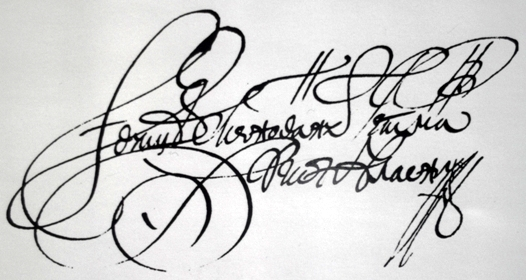
\includegraphics[width=1\linewidth]{4-1}}
\caption{Мини-рисунок, сделанный пользователем}
\label{ris:4.1}
\end{figure} 
